\chapter{はじめに}

\section{開発背景}

近年,PC,サーバ,組込みシステム等,用途を問わずマルチプロセッサの利用が進んでいる.
その背景には,シングルプロセッサの高クロック化による性能向上効果の限界や,消費電力・発熱の増大がある.
マルチプロセッサシステムでは処理の並列性を高めることにより性能向上を実現するため,消費電力の増加を抑えることができる.
組込みシステムにおいては,機械制御とGUIなど要件の異なるサブシステム毎にプロセッサを使用する例があるなど,従来から複数のプロセッサを用いるマルチプロセッサシステムが存在していたが,部品点数の増加によるコスト増を招くため避ける方向にあった.
しかしながら,近年は,1つのプロセッサ上に複数の実行コアを搭載したマルチコアプロセッサの登場により低コストで利用することが可能になり,低消費電力要件の強い,組込みシステムでの利用が増加している.

マルチプロセッサ環境でソフトウェアを開発する際に問題になる点として,デバッグの困難さが挙げられる.
これは,処理の並列性からプログラムの挙動が非決定的になり,バグの再現が保証されないため,シングルプロセッサ環境で用いられているブレークポイントやステップ実行を用いた従来のデバッグ手法が有効でないからである.

一方,マルチプロセッサ環境で有効なデバッグ手法として,プログラム実行履歴であるトレースログを解析する手法が挙げられる.
この手法が有効である理由は,並列プログラムのデバッグにおいて必要な情報である,各プロセスが,いつ,どのプロセッサで,どのくらい動作していたかということを,トレースログを解析することで知ることができるからである.
しかしながら,開発者が直接トレースログを解析するのは効率が悪い.
これは,膨大な量となるトレースログから所望の情報を探し出すのが困難であることや,各プロセッサのログが時系列に分散して記録されるため,逐次的にログを解析することが困難であることが理由である.

しかしながら,トレースログを開発者が直接扱うのは困難である場合が多い.
これは,ログの情報の粒度が細かくなるほど単位時間あたりのログの量が増える傾向にあり,膨大なログから所望の情報を探し出すのが困難であることや,各コアのログが時系列に分散して記録されるため,逐次的にログを解析することが困難であるからである.
そのため,トレースログの解析を支援するツールが要求されており,ログを解析し統計情報として出力したり,可視化表示することで開発者の負担を下げる試みが行われている.

\section{既存のトレースログ可視化ツール}

既存のトレースログ可視化表示ツールとしては,組込みシステム向けデバッガソフトウェアや統合開発環境の一部,Unix系OSのトレースログプロファイラ,波形表示用ツールの流用などがある.

本節では,これら既存のトレースログ可視化ツールについて説明した後,これらの問題点について指摘する.

\subsection{組込みシステム向けデバッガソフトウェア}

組込みシステム向けデバッガソフトウェアには,機能の1つとしてトレースログを可視化する機能が含まれている場合がある.
組込みシステム向けデバッガソフトウェアとは,ICE(In-Circuit Emulator)やJTAGエミュレータなどの,組込みシステム向けデバッガに付属するデバッグ用のソフトウェアである.
組込みシステム向けデバッガとは,ターゲットシステム上で動くプログラムをホストシステム上でデバッグを行えるようにするために,ターゲットCPUにアクセスする手段を提供する装置を指す.

組込みシステム向けデバッガソフトウェアとしては,京都マイクロコンピュータ株式会社のPARTNER\cite{PARTNER-JET}や,株式会社ソフィアシステムズのWatchPoint\cite{watchpoint}などがあり,それぞれ,イベントトラッカー,OSアナライザというトレースログを可視化する機能を提供している.
図\ref{fig:PARTNER-JET}に,イベントトラッカーのスクリーンショットを,図\ref{fig:watchpoint}にOSアナライザのスクリーンショットを示す.

これら組込みシステム向けデバッガソフトウェアの一機能としての可視化ツールは,その性質からターゲットとなるOSやプロセッサが限定される.
これは,組込みシステム向けデバッガは,通常,ターゲットとなるプロセッサが限られており,デバッガソフトウェアが対応するOSも限られているからである.
また,可視化表示したい情報も提供されているものに限られるなど,可視化ツールとしては汎用性,拡張性に乏しい.

\begin{figure}[p]
\begin{center}
\includegraphics[height=9cm]{img/PARTNER-JET.eps}
\caption{PARTNER イベントトラッカー}
\label{fig:PARTNER-JET}
\end{center}
\end{figure}

\begin{figure}[p]
\begin{center}
\includegraphics[height=4cm]{img/watchpoint.eps}
\caption{WatchPoint OSアナライザ}
\label{fig:watchpoint}
\end{center}
\end{figure}

\subsection{組込みOS向けの統合開発環境}

QNX Software Systems社は,自社の組込みリアルタイムオペレーティングシステムQNXの統合開発環境としてQNX Momenticsを販売している.QNX Momenticsにはシステムプロファイラとして,システムコールや割込み,スレッド状態やメッセージなどを可視化するQNX System Profiler\cite{QNXMomentics}という機能を提供している.図\ref{fig:QNXSystemProfiler}にQNX System Profilerのスクリーンショットを示す.

また,イーソル株式会社はT-Kernel/$\mu$ITRONベースシステムの統合開発環境としてeBinder\cite{eBinder}を販売している.eBinderにはイベントログ取得・解析ツールとしてEvenTrekが付属しており,システムコール,割込み,タスクスイッチ,タスク状態遷移などを可視化することができる.図\ref{fig:EvenTrek}にEvenTrekのスクリーンショットを示す.

このように,商用の組込みOS向けの統合開発環境にはOSの実行履歴を可視化表示する機能が搭載されている場合がある.しかしながら,これらは,各ベンダーが自社OSの競争力を高めるために提供しているものであり,当然ながら可視化表示に対応するOSは自社提供のものに限られている.
また,可視化表示する情報も提供するものに限られており,表示のカスタマイズ機能もそれほど自由度は高くはない.

\begin{figure}[p]
\begin{center}
\includegraphics[height=9cm]{img/QNXSystemProfiler.eps}
\caption{QNXSystemProfiler}
\label{fig:QNXSystemProfiler}
\end{center}
\end{figure}

\begin{figure}[p]
\begin{center}
\includegraphics[height=9cm]{img/EvenTrek.eps}
\caption{eBinder EvenTrek}
\label{fig:EvenTrek}
\end{center}
\end{figure}

\subsection{Unix系OSのトレースログプロファイラ}

Unix系OSでは,これまでに,パフォーマンスチューニングや障害解析を目的として,カーネルの実行トレースを取得するソフトウェアがいくつか開発されている.
ここでは,単にこれをトレースツールと呼称する.

Linux用のトレースツールとしてはLKST\cite{LKST},SystemTap\cite{SystemTap},LTTng\cite{LTTng}などがあり,Solaris用にはDtrace\cite{Dtrace}がある.
これらトレースツールが提供する主な機能は,カーネル内にフックを仕込みカーネル内部状態をユーザー空間に通知する機能と通知をログとして記録する機能である.

これらのトレースツールは,ログを分析,提示する,専用のプロファイラツールを提供している場合が多い.
たとえば,LTTngにはLTTV\cite{LTTV}が,DTraceにはChime\cite{Chime}が,プロファイラツールとして提供されている.
図\ref{fig:LTTV}にLTTVのスクリーンショットを,図\ref{fig:Chime}にChimeのスクリーンショットを示す.

これら,プロファイラツールは,主に,カーネルの内部状態を統計情報として出力することにより,ボトルネックを探したり,障害の要因を探る目的で使用されるが,ソフトウェアのデバッグを目的に使用することもできる.
DTraceなどはログ出力のためのカーネルフックポイントを独自のスクリプト言語を用いて制御できるなど,任意の情報をソフトウェアの実行から取得することができる.
しかしながら,取得したログを任意の図形で可視化する手段は提供されておらず,テキスト形式での確認となる.
また,可視化表示する際のログの形式は,そのOSのトレースツールが出力する形式に依存するため,他のOSのトレースを可視化することはできない.

\begin{figure}[p]
\begin{center}
\includegraphics[height=9cm]{img/LTTV.eps}
\caption{LTTV}
\label{fig:LTTV}
\end{center}
\end{figure}

\begin{figure}[p]
\begin{center}
\includegraphics[height=9cm]{img/Chime.eps}
\caption{Chime}
\label{fig:Chime}
\end{center}
\end{figure}

\subsection{波形表示ツールの流用}

任意のOS,アプリケーションのトレースログを可視化表示する手段として,波形表示ツールを流用する方法がある.
波形表示ツールとは,Verilog等のデジタル回路設計用論理シミュレータの実行ログを波形で表示するソフトウェアのことを指す.

デジタル回路設計用論理シミュレータの実行ログには,VCD(Value Change Dump)形式というオープンなファイルフォーマットが存在する.
そのため,任意のログをVCD形式として出力することにより,これらのツールで可視化表示することが可能になる.
図\ref{fig:GTKWave}に,VCD形式のログの可視化に対応した波形表示ツールGTKWaveのスクリーンショットを示す.

波形表示ツールを流用する方法では,任意のログをオープンフォーマットなファイル形式に変換することによりログの形式に依存せずに利用できる反面,表示能力に乏しく,複雑な可視化表現は難しいという問題がある.

\begin{figure}[t]
\begin{center}
\includegraphics[height=9cm]{img/GTKWave.eps}
\caption{GTKWave}
\label{fig:GTKWave}
\end{center}
\end{figure}

\subsection{既存のトレースログ可視化ツールの問題点}

既存のトレースログ可視化ツールは,可視化ツールとして単体で存在しているわけではなく,トレースログを出力するソフトウェアの一部として提供されている.
そのため,読み込めるトレースログの形式が出力ソフトウェアに依存しており,可視化対象となるOS,プロセッサが制限されてしまっている.

読み込むトレースログの形式を制限しないためには,波形表示ツールのようにトレースログ可視化ツール用に標準化されたトレースログ形式を定める必要があると考えられるが,現状,公表されているものではそのようなものは確認できていない.

ログ形式の標準化としては,syslog\cite{RFC3164}と呼ばれる,ログメッセージをIPネットワーク上で転送するための標準規格がRFC3164として策定されており,その一部にログ形式について規定されている.
しかしながら,syslogにおけるログ形式は,時刻の最小単位が秒であり,デバッグを目的に利用するには粒度が粗く,また,メッセージ内容がフリーフォーマットであるなど,自由度が高すぎるため,可視化ツールが読み込むログの標準形式としては不適切である.

既存のトレースログ可視化ツールのもうひとつの問題点としては,可視化表示の項目や形式が,提供されているものに限られていることが挙げられる.
既存のトレースログ可視化ツールで可視化表示の項目を追加,変更したり,可視化表現をカスタマイズする機能を搭載するものは確認できていない.

\section{開発目的と内容}

前節で説明したとおり,既存のトレースログ可視化ツールには,標準化されたトレースログ形式がないことによりターゲットが限定されてしまっているという,汎用性に乏しい点と,可視化表示項目が提供されているものに限られているという,拡張性に乏しい点の2つの問題点があることを指摘した.

そこで我々は,これらの問題点を解決し,汎用性と拡張性を備えたトレースログ可視化ツールを開発することを目的とし,TraceLogVisualizer (TLV) を開発した.

はじめに,TLVの内部でトレースログを抽象的に扱えるよう,トレースログを一般化した標準形式トレースログを定めた.
次に,任意の形式のトレースログを標準形式トレースログに変換する仕組みを変換ルールとして形式化した.
この変換ルールを外部ファイルとして与えることで,任意の形式のトレースログを読み込めるようになる.

また,トレースログの可視化表現を指示する仕組みを抽象化し,可視化ルールとして形式化した.
この可視化ルールも,同じように外部ファイルとして与えることで,可視化表示項目の追加や変更,可視化の表現方法を自由に設定することができるようになる.

TLVでは,このように,変換ルールと可視化ルールを外部ファイルとして与えることで,汎用性と拡張性を実現した.
これらの外部ファイルは,ユーザーが記述することを想定し,読み書きのしやすいシンタックスを持つJson(JavaScript Object Notation)\cite{Json}というデータ記述言語を採用し,ファイルの記述内容に合わせてセマンティクスを規定した.


\section{論文の構成}
本節では本論文の構成を述べる.

2章では,TLVの設計について述べる.
ここでは,問題解決のために開発方針をどのように設定したかを述べ,具体的な解決策をどのように設計したかを述べる.
3章では,TLVの実装について述べる.
2章で述べた設計をメカニズムとしてどのように実現しているかを説明する.
4章では,TLVを利用した例を示し,その有効性について言及している.
5章ではTLVを開発するにあたり,どのような開発プロセスを用いたのかを述べている.
最後に6章で本論文のまとめと今後の展望と課題について述べる.